\chapter{Introduction} 

%
The unique properties of organic semiconductors make them ideal candidates for
many electronic applications. They are used today in ultra high resolution \gls{oled} 
TVs and cellphone displays. They enable cutting edge
foldable \glsxtrshort{oled} screens and rollable TVs \cite{Chen2020}.
Organic semiconductors are also integral to the design of next generation medical devices owing to their
self-healing properties and their biodegradability \cite{Bettinger2010}. 
For more on bioelectronic materials, see Organic Electronic: Emerging Concepts and Technologies
\cite{FabioCicoiraEditor2013}.

In this thesis, we focus on a subclass of organic semiconductors, \gls{opv} materials, and their use in the
active layer of \gls{osc} devices.  
\glsxtrshort{osc}s, the reverse of the more popularly understood OLEDs,
are devices that absorb photonic energy and extract electronic energy. 
A rudimentary \gls{osc} is drawn in \autoref{bhj}.
We note that any organic semiconductor can exhibit a photovoltaic effect if a
photon with commensurate energy is incident on the material.
\glsxtrshort{opv}s are therefore distinguished by
their capacity for electronic energy level 
tuning and their ability to be processed into structures suitable to a given design purpose.

\glsxtrshort{osc}s exhibit improvements in
flexibility, processability, and cost of manufacturing.
They are also used in more revolutionary electronic designs.
For example, researchers have exploited the relatively narrow absorption spectrum in \glsxtrshort{opv}s
(${\sim}300nm$) to make windows that act as OSCs. 
They achieved this by tuning the active layer material to absorb radiation right above or right below the
visible spectrum (into the NIR or UV spectrum respectively). 
Semi-transparent \glsxtrshort{osc}s have already
reached 11 \% efficiency \cite{Brabec2020}. 

OSCs are approaching 20\% efficiency \cite{Liu2020b}.
Two major breakthroughs have ushered us into the modern era of \glsxtrshort{osc}s.
These are the design of \gls{bhj} active layers and non-fullerene, \gls{frea} molecules. 

A fundamental physical difference in the nature of photoabsorbtion in inorganic and organic 
semiconducting materials necessitated the
invention of the \glsxtrshort{bhj}. The coulombic attraction, $V$, between an excited
electron and the hole it leaves behind in the its molecular orbital
is given by Coulombs law as follows:
\begin{align}
    \label{coulomb}
    V  = k_{e} \cdot \frac{e^{2}}{\epsilon_{r}}
\end{align}
where $k_{e}$ is Coulomb's constant and $e$ is charge of an electron. Relative
permittivity,
$\epsilon_{r}$, is a unitless quantity that describes a materials polarizability relative
to that of free space. That is, relative
permittivity describes the readiness of a material
to polarize in response to an electric field. A low
relative permittivity of ${\sim}3$ in \glsxtrshort{opv}s (${\sim}12$ for silicon \cite{Baroni1986} and ${\sim}78$ for water \cite{George2004})
means that these materials are only $3$ times more polarizable than free space, which
is not all that polariazable. And, because the material occupying the space between electron and hole
is not willing (or able?) to fight back against the electric field created between them, they stick together and behave as a quasipartcle. 
This bound electron-hole quasiparticle is referred to herein as an exciton.

% keep attachced to prior paragraph
This excitonic absorption introduces a unique design challenge.
That is, to extract a charge from the device, the exciton
must first be coerced apart. This coercion can take place at the interface between donor and acceptor molecules,
where the slight offset in energy levels creates a charge transfer state wherein it is more
energetically favorable for the donor to undergo electron transfer with an adjacent acceptor than
it is to radiatively decay to its ground state and photoemit.
This means that, after photoabsorbtion, the exciton must to diffuse to this interface for the charge to be
extracted. Because an exciton can only diffuse so far (${\sim}10nm$ \cite{clarke2010}) before it relaxes to
its ground state, it is critical that absorption take place close to a donor/acceptor
interface. 
Producing extremely thin active layers could conceivably achieve this. However,
producing a layer this small is untenable from a manufacturing standpoint. Furthermore, extremely thin active
layers restrict the amount of radiation that a device interacts with. 

In 1986, Ching W. Tang
showed that, processed under the right conditions, a blend of donor and acceptor molecules can self-assemble
into a \glsxtrshort{bhj} microstructure \cite{Tang1986c}. 
The interlocking phases of donor accepter molecules, ensure
that an exciton will intersect with the boundary between accepter and donor domains, while also ensuring that
there
is a continuous escape route, albeit labyrinthine, for the free charges to travel on their way to their respective
electrodes. 

\begin{figure}
    \center
    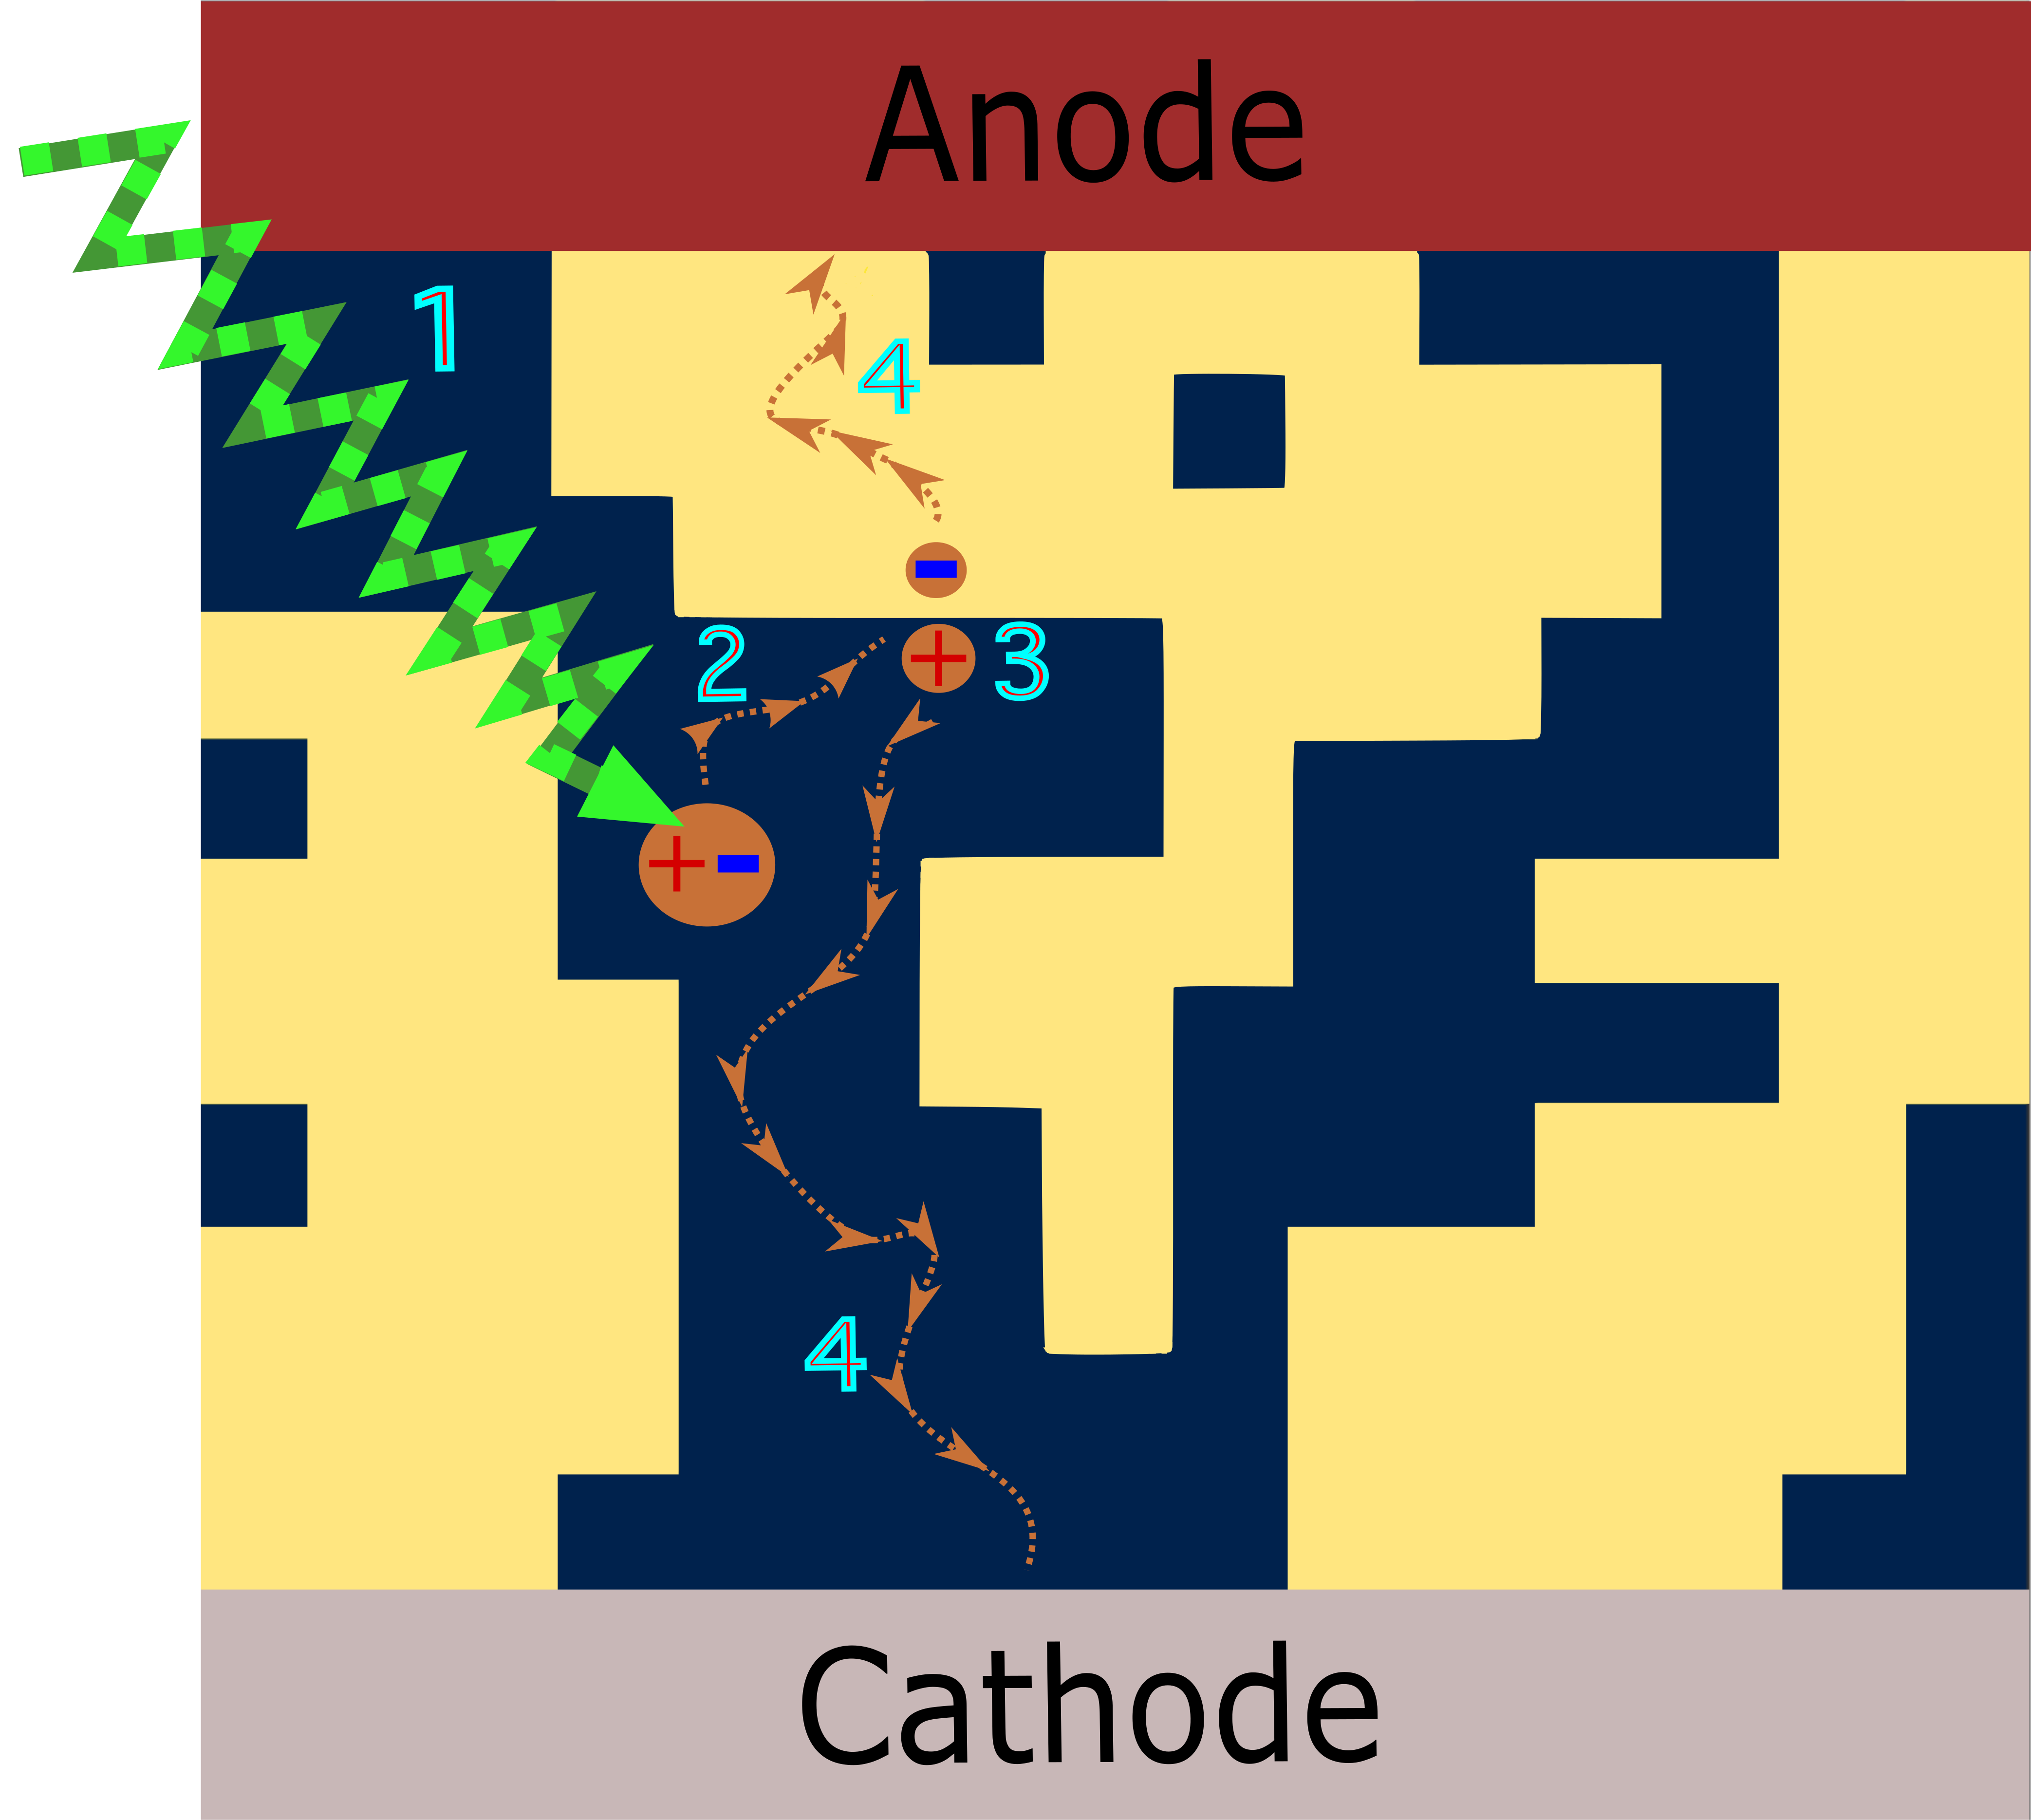
\includegraphics[width = .6\textwidth]{figures/BHJ-figure.png}
    \caption{A cartoon representation of a \glsxtrshort{bhj} device. All four stages involved in harvesting
    photonic energy in a \glsxtrshort{bhj} device are represented. (1) The photon (green arrow) interacts with the material,
    exciting an electron and creating an quasiparticle referred to as an exciton. (2) The exciton diffuses
    about until it intersects the interface between donor and acceptor material domains. (3) The exciton is
    coerced apart by the energy offset between donor and acceptor molecules. 
    (4) The, now unbound,  hole and the electron are free to diffuse about until they reach their respective
    electrodes where they can be extracted \cite{Fusella2019}.}
    \label{bhj}
\end{figure}

% Keep attached to prior paragraph.

As shown in \ref{bhj}, a \glsxtrshort{bhj} active layer is designed to harvest photons through the following 
steps: (1) photoabsorbtions, 
(2) exciton diffusion, (3) charge transfer, and (4) free charge diffusion \cite{Fusella2019}. 
When a photon is incident on
an \glsxtrshort{osc} active layer, if it intersects with a molecular segment in the donor whose 
\gls{homo} has comparable energy levels to the photon, 
the energy can be absorbed via the promotion of
an electron to the next available energy level; the \gls{lumo}.
This forms an exciton as
described above, which can then diffuse until it intersects the boundary. 
The excited electron would like to relax
back into is lower energy level, but at the interface with the acceptor, it finds a better option. The
acceptor's \glsxtrshort{lumo} is engineered to sit between the energy of the donor's excited electron's energy level and the
available lower energy level. Because of this, the electron cascades down to the acceptors \glsxtrshort{lumo} through a charge
transfer reaction. Finally the free charges can diffuse until they interact the electrode where it can be
extracted. This is, of course, an ideal description, as there are loss mechanisms at all four stages. 

The \glsxtrshort{bhj} design pushed the efficiency beyond the 1\% milestone. However, early \glsxtrshort{bhj} devices utilized
fullerene derivatives as acceptors which have a theoretical efficiency limit of $\sim13\%$ \cite{Scharber2016}
and their spherical
structure leads to difficult chemical purification, weak absorption in the visible-NIR spectrum, and rapid
device degradation. In 2015, a group of researchers conceptualized the use of
\gls{frea}s. \glsxtrshort{frea}s consist of
a fused-ring core and end groups that can be engineered to achieve specific electronic characteristics and side
chains that can be engineered to achieve desired morphological features. The modularity of \glsxtrshort{frea}s
laid the stage for headspinning progress in the following years from 4\% efficiency to 18\% 
efficiency~\cite{Wang2021a}. 
This designed modularity is a benefit to researchers, as they can alter one moiety and test
the effect on resulting charge characteristics. For example, in a paper published in 2019 \cite{Benatto2019},
researchers, knowing that flourine is an electronegative atom, swapped 4 hydrogen atoms for flourine atoms on
the end groups the \glsxtrshort{frea} molecule \glsxtrshort{itic}. Using \textit{ab initio} DFT, they found 
that this substitution could lower the exciton
binding energy (discussed above using \autoref{coulomb}), thus facilitating exciton disassociation (stage 3 of
\glsxtrshort{bhj}). They also found
that this flourination tends to reduce the reorganization energy, which we see
in \autoref{results}, drastically increases charge mobility.

Our work in this thesis
is most expressly related to stage $4$ of charge photogeneration in \gls{bhj} active layers.
We simulate the self-assembly and charge mobility of pure acceptor (or
pure donor) domains post deposition. 
How the materials will self-assemble in the environment in which they are deposited determines
the morphology which intern governs charge mobility \cite{McMahon2011}. 
With that, we outline the data pipeline in \autoref{pipeline}, through which we take atomistic representations like
those shown in \autoref{molecules} and, through a series of computations and simulations,
arrive at data that is predictive of material properties. 
This pipeline is laid out in further detail by Jones et al.~\cite{jones2017}.
The pipeline begins with an atomistic description of a given molecule's atom types and bonding structure.
On the basis of this description, forces between all atoms are defined. On the basis of these interacting
forces, equilibrium \gls{md} simulations can predict the morphological structure. 
The structural data obtained from these simulations can then be fed as an input into \gls{kmc}
simulations that characterize charge mobility (conductivity) in these chemistries based on the
energetics of electronically active molecular segments (`chromophores') within the morphology.
We \texttt{Planckton}, our package for navigation MD simulations of \glsxtrshort{opv}S in \autoref{planckton}. 
The focus of this thesis, however, is the development of \texttt{MorphCT} for running \glsxtrshort{kmc} simulations, which we
introduce more thoroughly in \autoref{morphct}.

\begin{figure}
  \center
  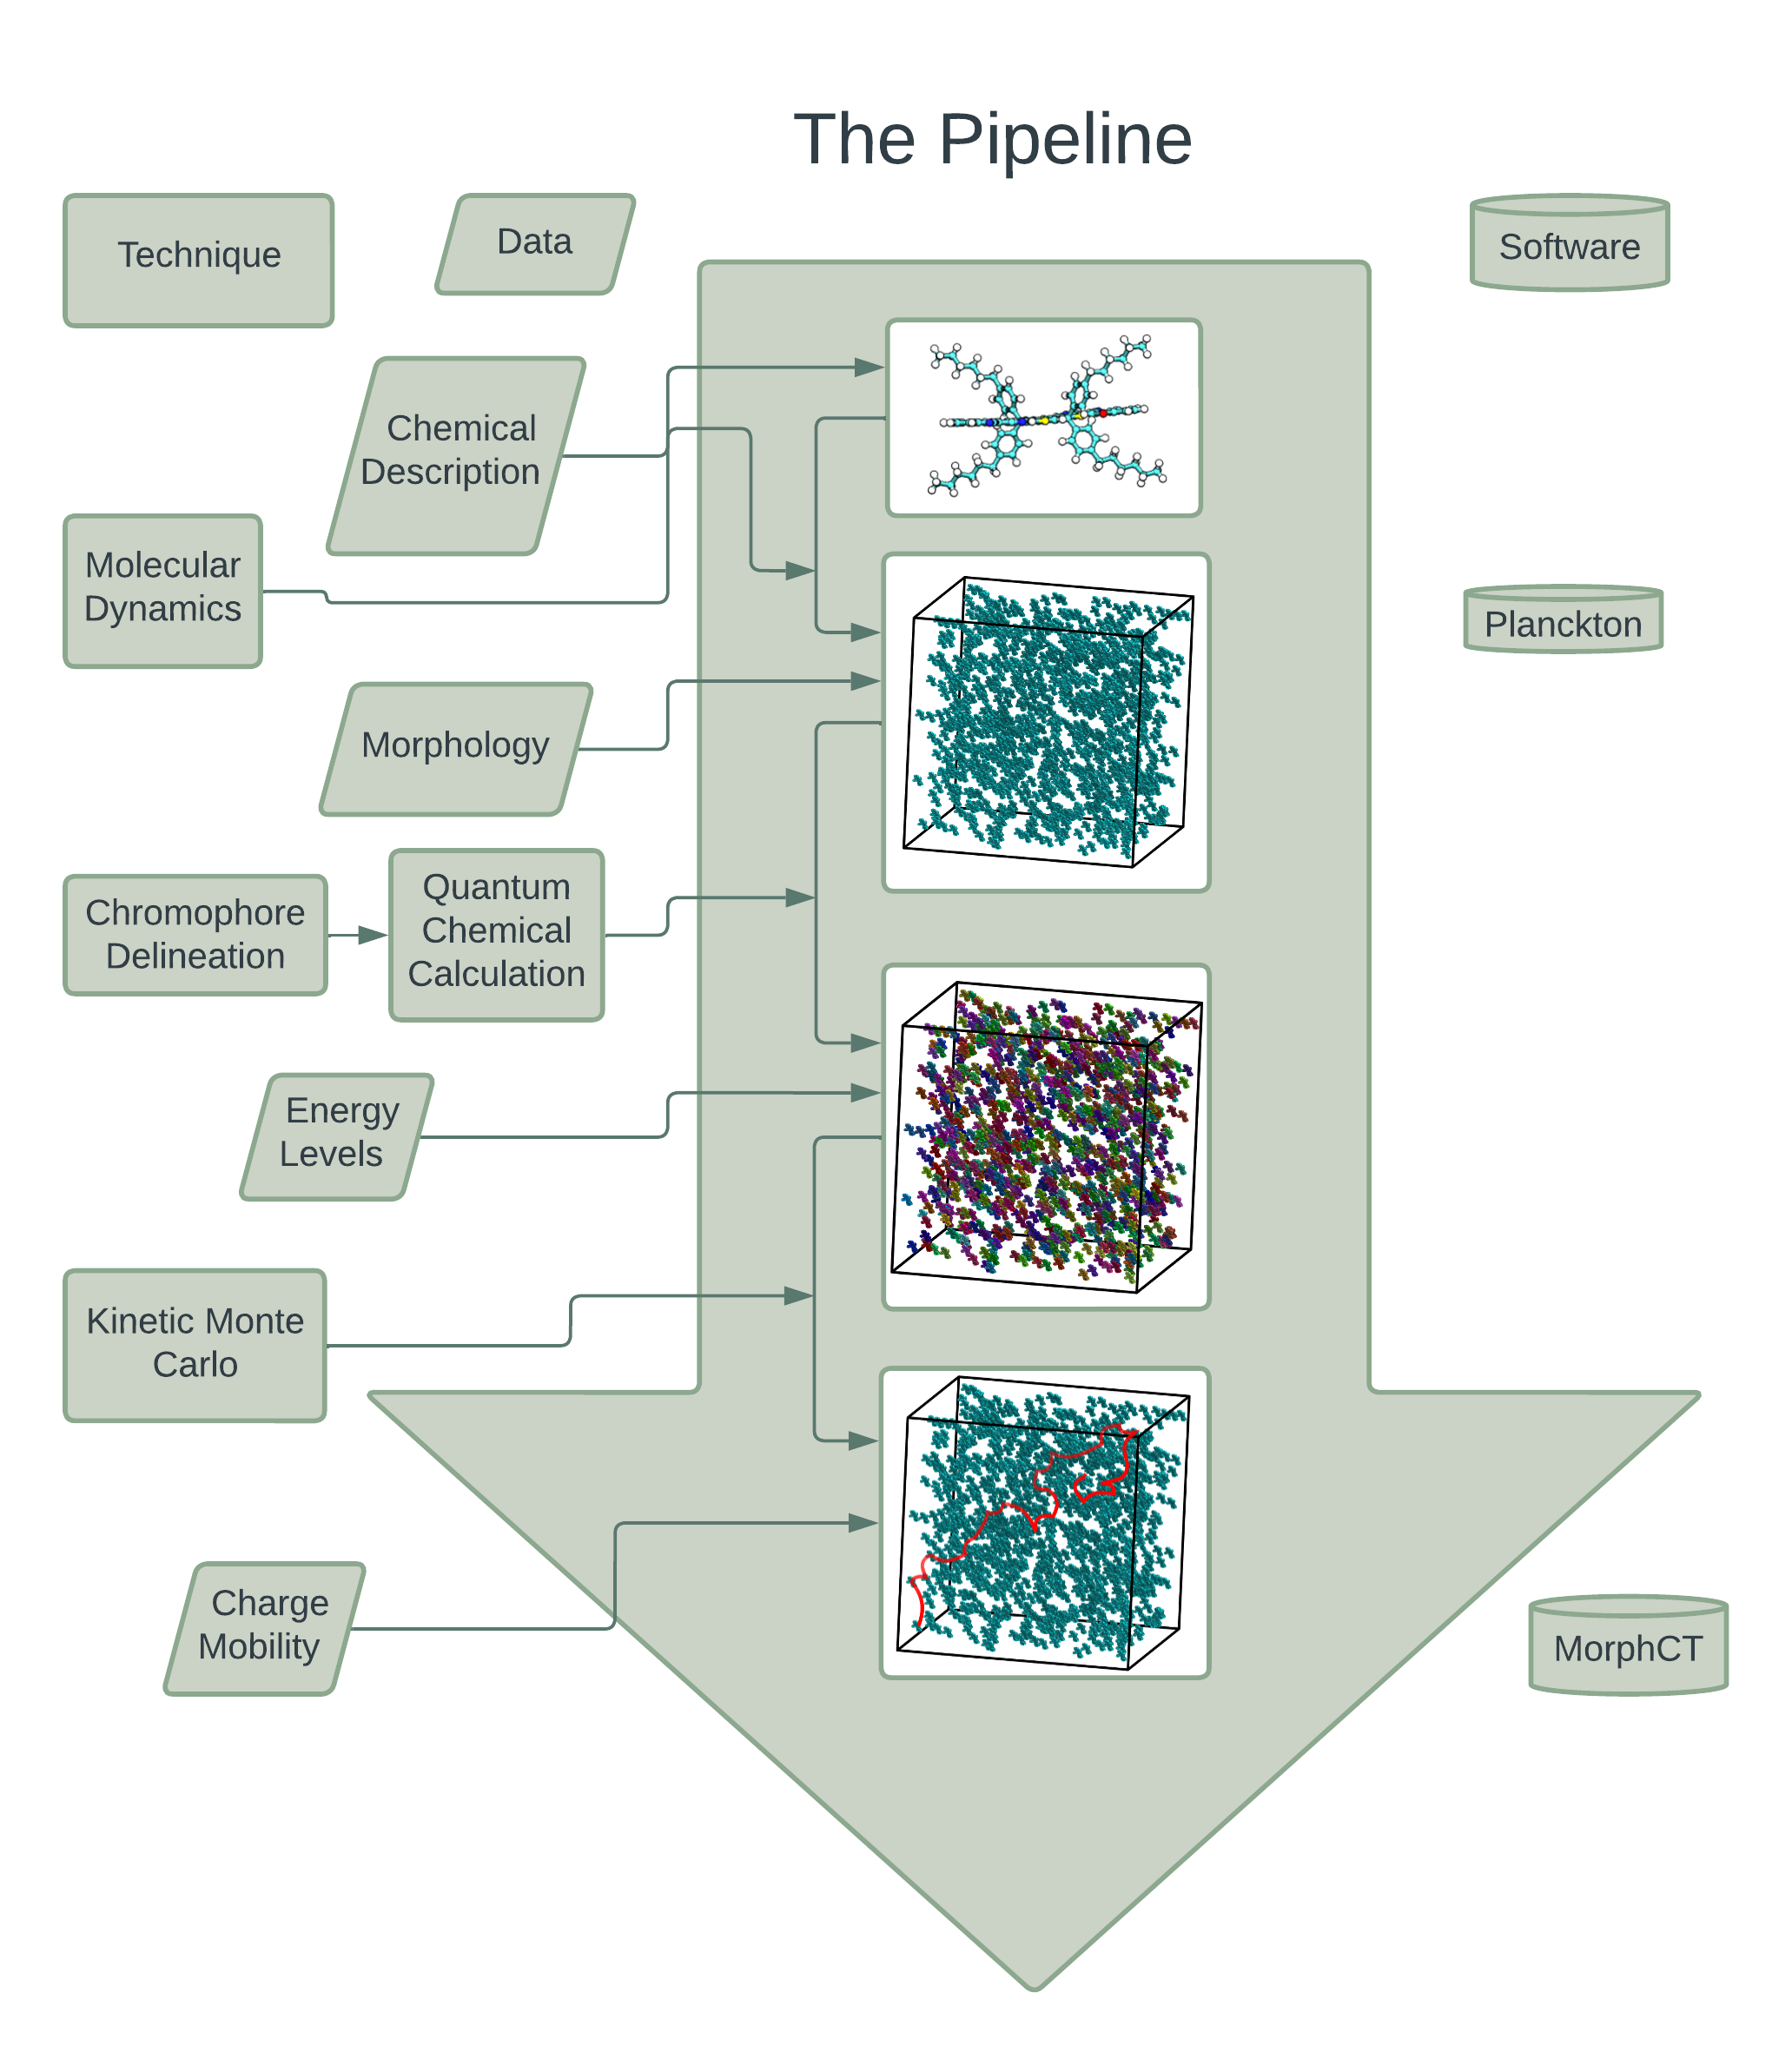
\includegraphics[width=0.9\linewidth]{figures/the-pipeline.png} 
    \caption{The pipeline for progressively graduating atomistic data to charge characteristics. On the left
    we see our packages developed for navigating the pipeline.}
  \label{pipeline}
\end{figure}

We use the term `chromophore' liberally in this thesis. We take a brief aside to be more
explicit about its meaning.  
The term chromophore arose in a biochemical context and is generally defined
as a light-absorbing group or molecule \cite{biochemistry}.
In this context, a chromophore is so named because these molecules are associated with the color of a material.
This is because, mechanistically, a photon collides with a chromophore, the absorbed energy
excites an electron from the \glsxtrshort{homo} to the
\glsxtrshort{lumo}. When the chromophore relaxes to its
ground state, it releases a photon with wavelength (or color) $\lambda = \frac{\hbar c}{E}$,
where $\hbar$ is Plank's constant, $c$ is the speed of light, and $E$ represents the
energy difference between the \glsxtrshort{homo} and \glsxtrshort{lumo}. 
In plants, this amounts to a rejection of the overabundant amount of
light in the green region which can damage the plant's DNA. 
We continue with the use of the term chromophore
for the sake of brevity. In what is to follow, chromophore is taken to be defined as a molecular segment over which the 
wave function of a free electron (hole) is assumed to be localized.
It is under this assumption that we execute a hopping model of charge transfer between
chromophores based on the Marcus rates of electrochemical reactions. We will also use chromophore to refer to
the object in computer memory that stores all the information that we know about a chromophore within morphology
(e.g., atom locations, neighbors, energy levels).

%%In \autoref{results} we explore the delineation of these localiztion segments for simulation, which we hereafter refer to as a `chromophore.' 

Engineering the charge mobility of pure donor and acceptor domains is critical
to overall device performance \cite{Wang2019e}.
An understanding of why this is the case can be found from the inspection of \autoref{bhj}.
If the electrons in stage $4$ reach the anode much faster than the holes reach the cathode, a traffic jam can
occur at the anode which can result in recombination with surrounding holes and ultimately a loss of the
charge via annihilation. 
The imbalanced charge carrier mobility can also lead to space-charge build up in the 
low mobility material that can screen the built in field~\cite{Bartelt2015}.
This phenomena has been shown by space charge limited current experiments~\cite{Small2013}.

To improve the efficacy of the pipeline we focus on
developing simulation tools are that are
\gls{true} (\cite{Cummings2017}).
With scientific research being an innately distributed endeavor, these virtues provide a lens through which to
evaluate the adherence to basic scientific principles and to the best practices of distributed software development
simultaneously. As enumerated by Jankowski et al., some of emerging best practices for scientific software
development include the following: (1) address cognitive load, (2) use version control, (3) automate
repetitive tasks, (4) develop open-source code, (5) write code in the highest language possible~\cite{Jankowski2020}.
`Addressing cognitive load' amounts to an admission that a learner has a
finite capacity for new ideas~\cite{Jankowski2019}.
% SHOULD Say: Thesis summary. Add a sentence or two on each of (a) your thesis plan, (b) what you found, (c) what it means. 

We seek to improve the pipeline outlined in \autoref{pipeline}.
To do this, we: (1) integrate an open source quantum chemical package into \texttt{MorphCT},
(2) perform validation and sensitivity analysis on benchmark \glsxtrshort{p3ht}
morphologies and
(3) deploy the pipeline from start to finish on \glsxtrshort{itic}. 
Informing this work is a new developer's perspective on cognitive load. 
Two specific challenges to this work were (1) understanding which facets of quantum
theory were being applied, and (2) learning the application programming
interface of the \texttt{MorphCT}.
Tutorials, documentation, github issues, and searchable collaborative workspace
forums (Slack) provided a foundation for using and learning \texttt{MorphCT}.
We aim to address challenges (1) and (2) through the publication of interactive
Jupyter notebook tutorials.

\begin{figure}
\centering
\begin{subfigure}{.5\textwidth}
    \centering
    \textbf{(A)} \glsxtrshort{p3ht} \\
    \includegraphics[width=\textwidth]{figures/p3ht-molecule-figure.png}
\end{subfigure}%
\\
\begin{subfigure}{.3\textwidth}
    \textbf{(B)} \glsxtrshort{itic}
    \centering
    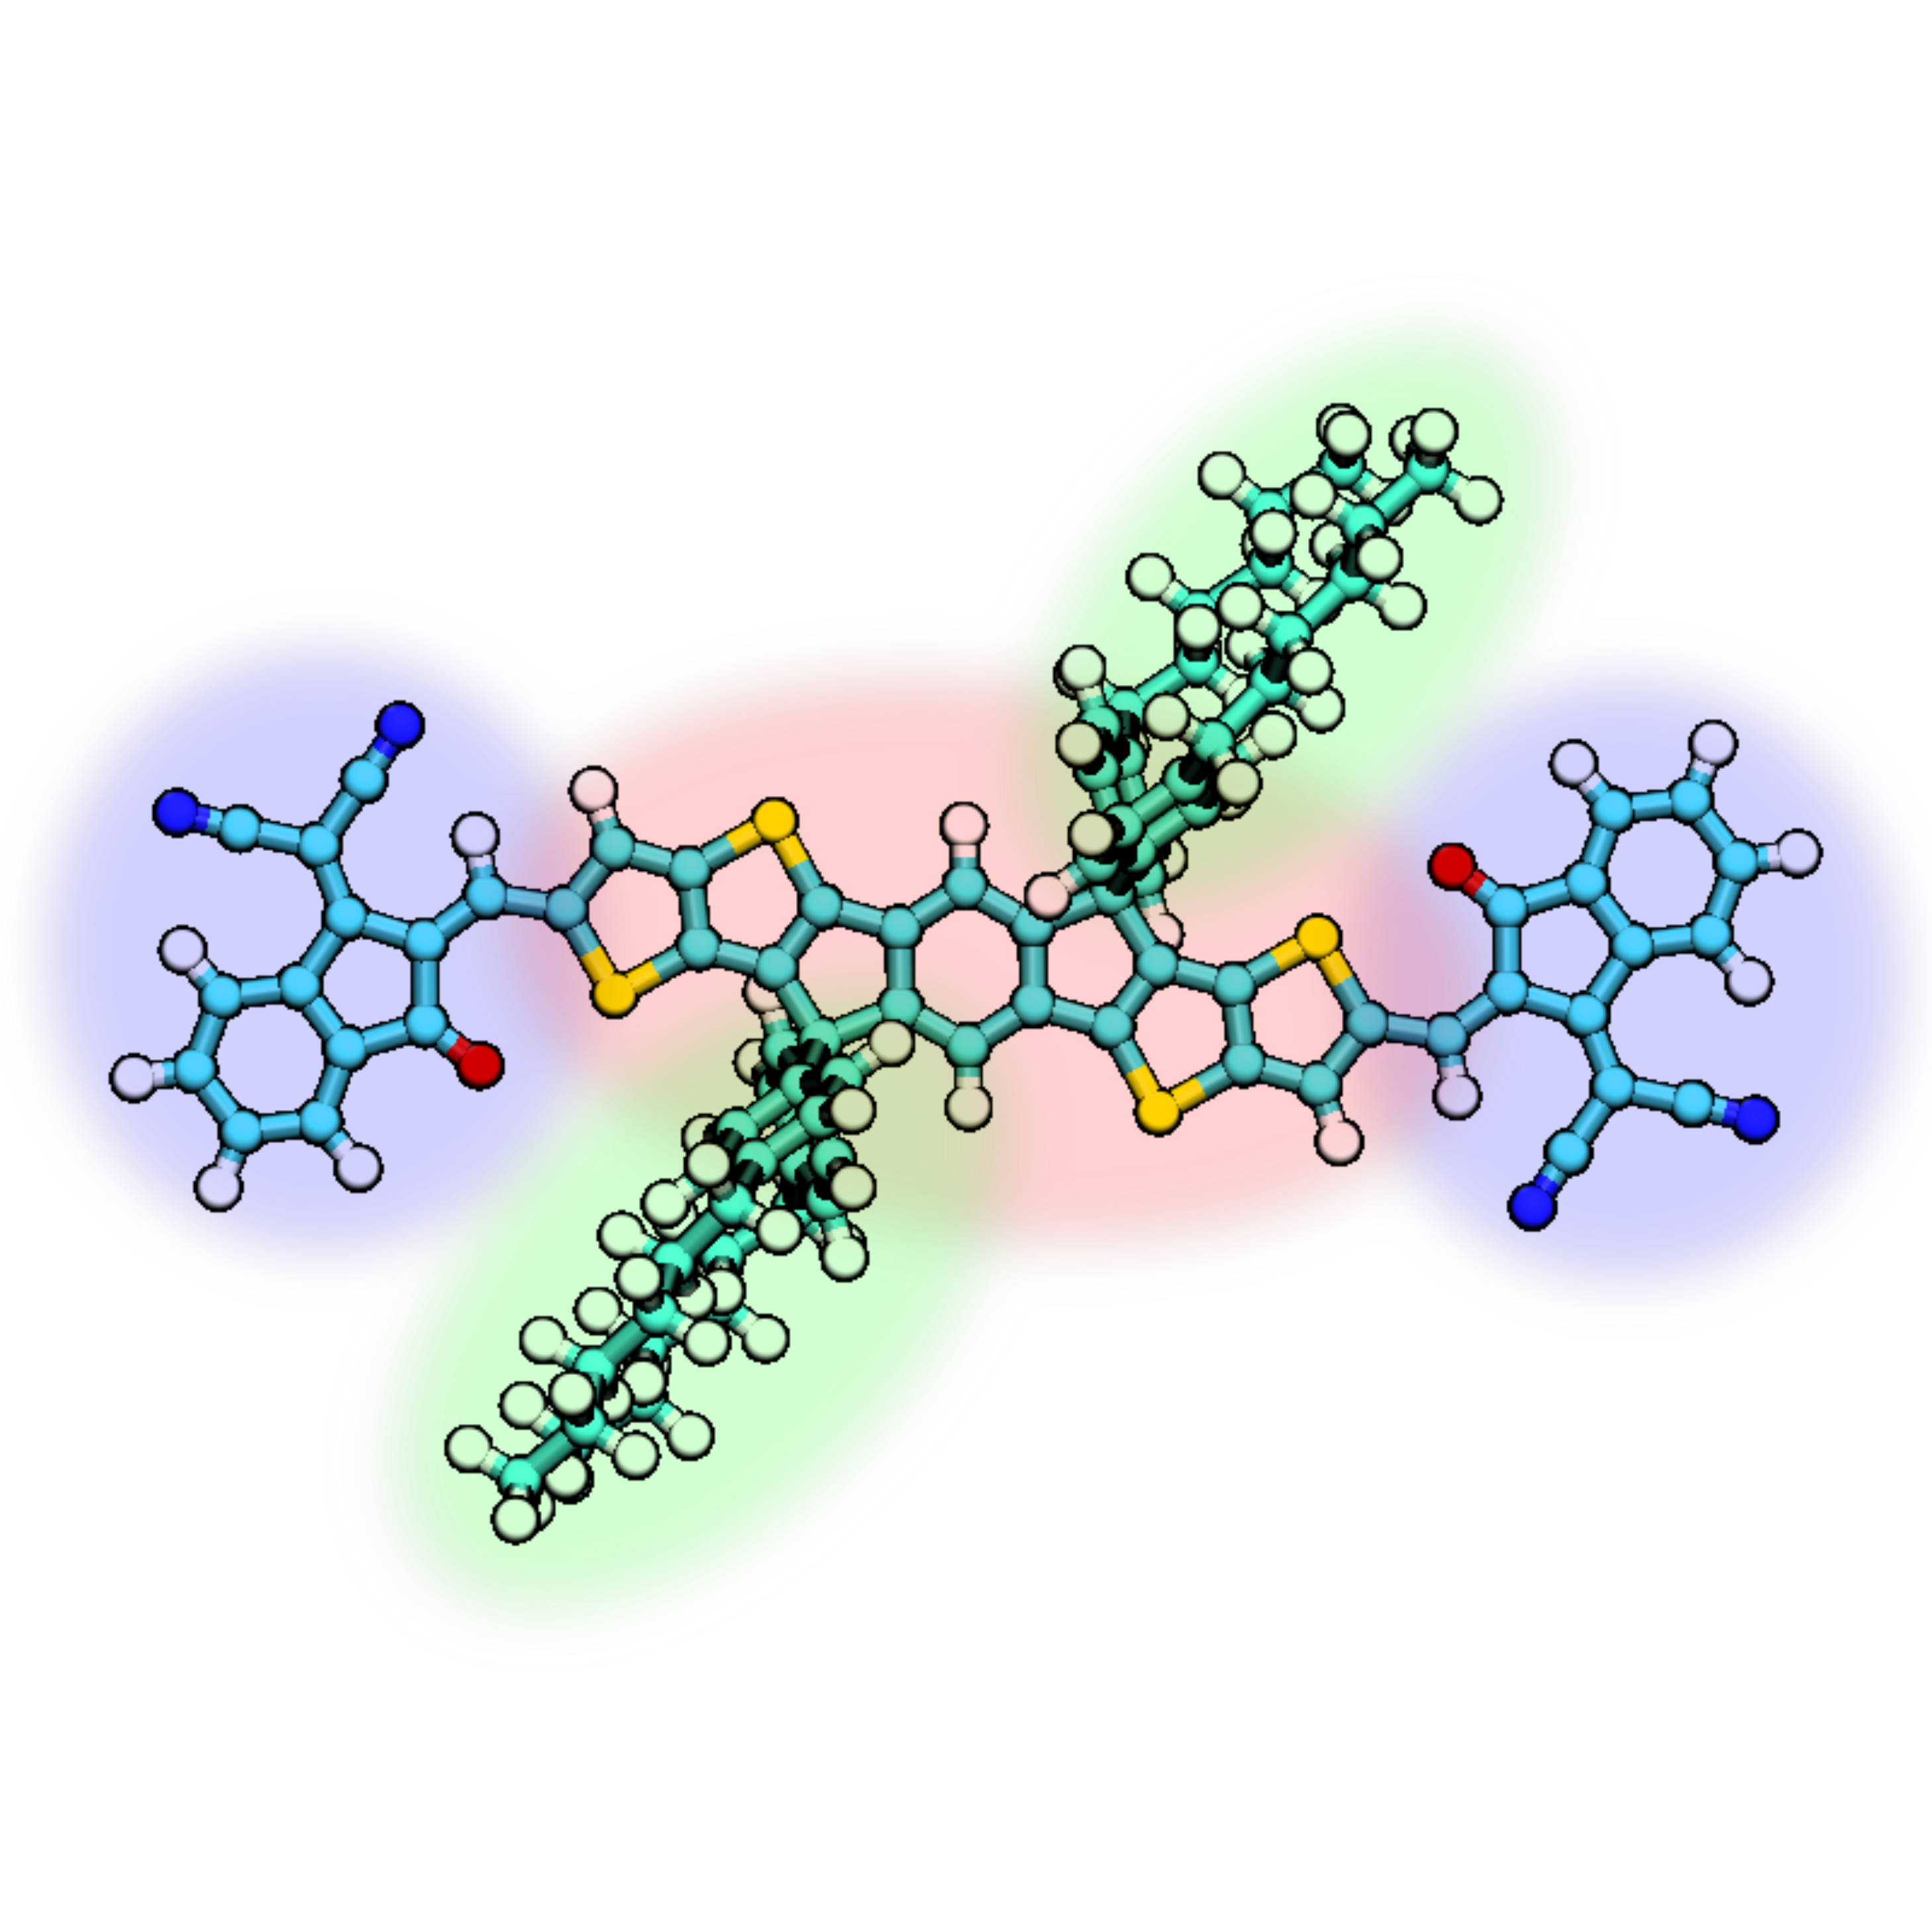
\includegraphics[width=\textwidth]{figures/itic-backbone-figure.png}
\end{subfigure}%
\begin{subfigure}{.3\textwidth}
    \textbf{(C)} \glsxtrshort{itic}
    \centering
    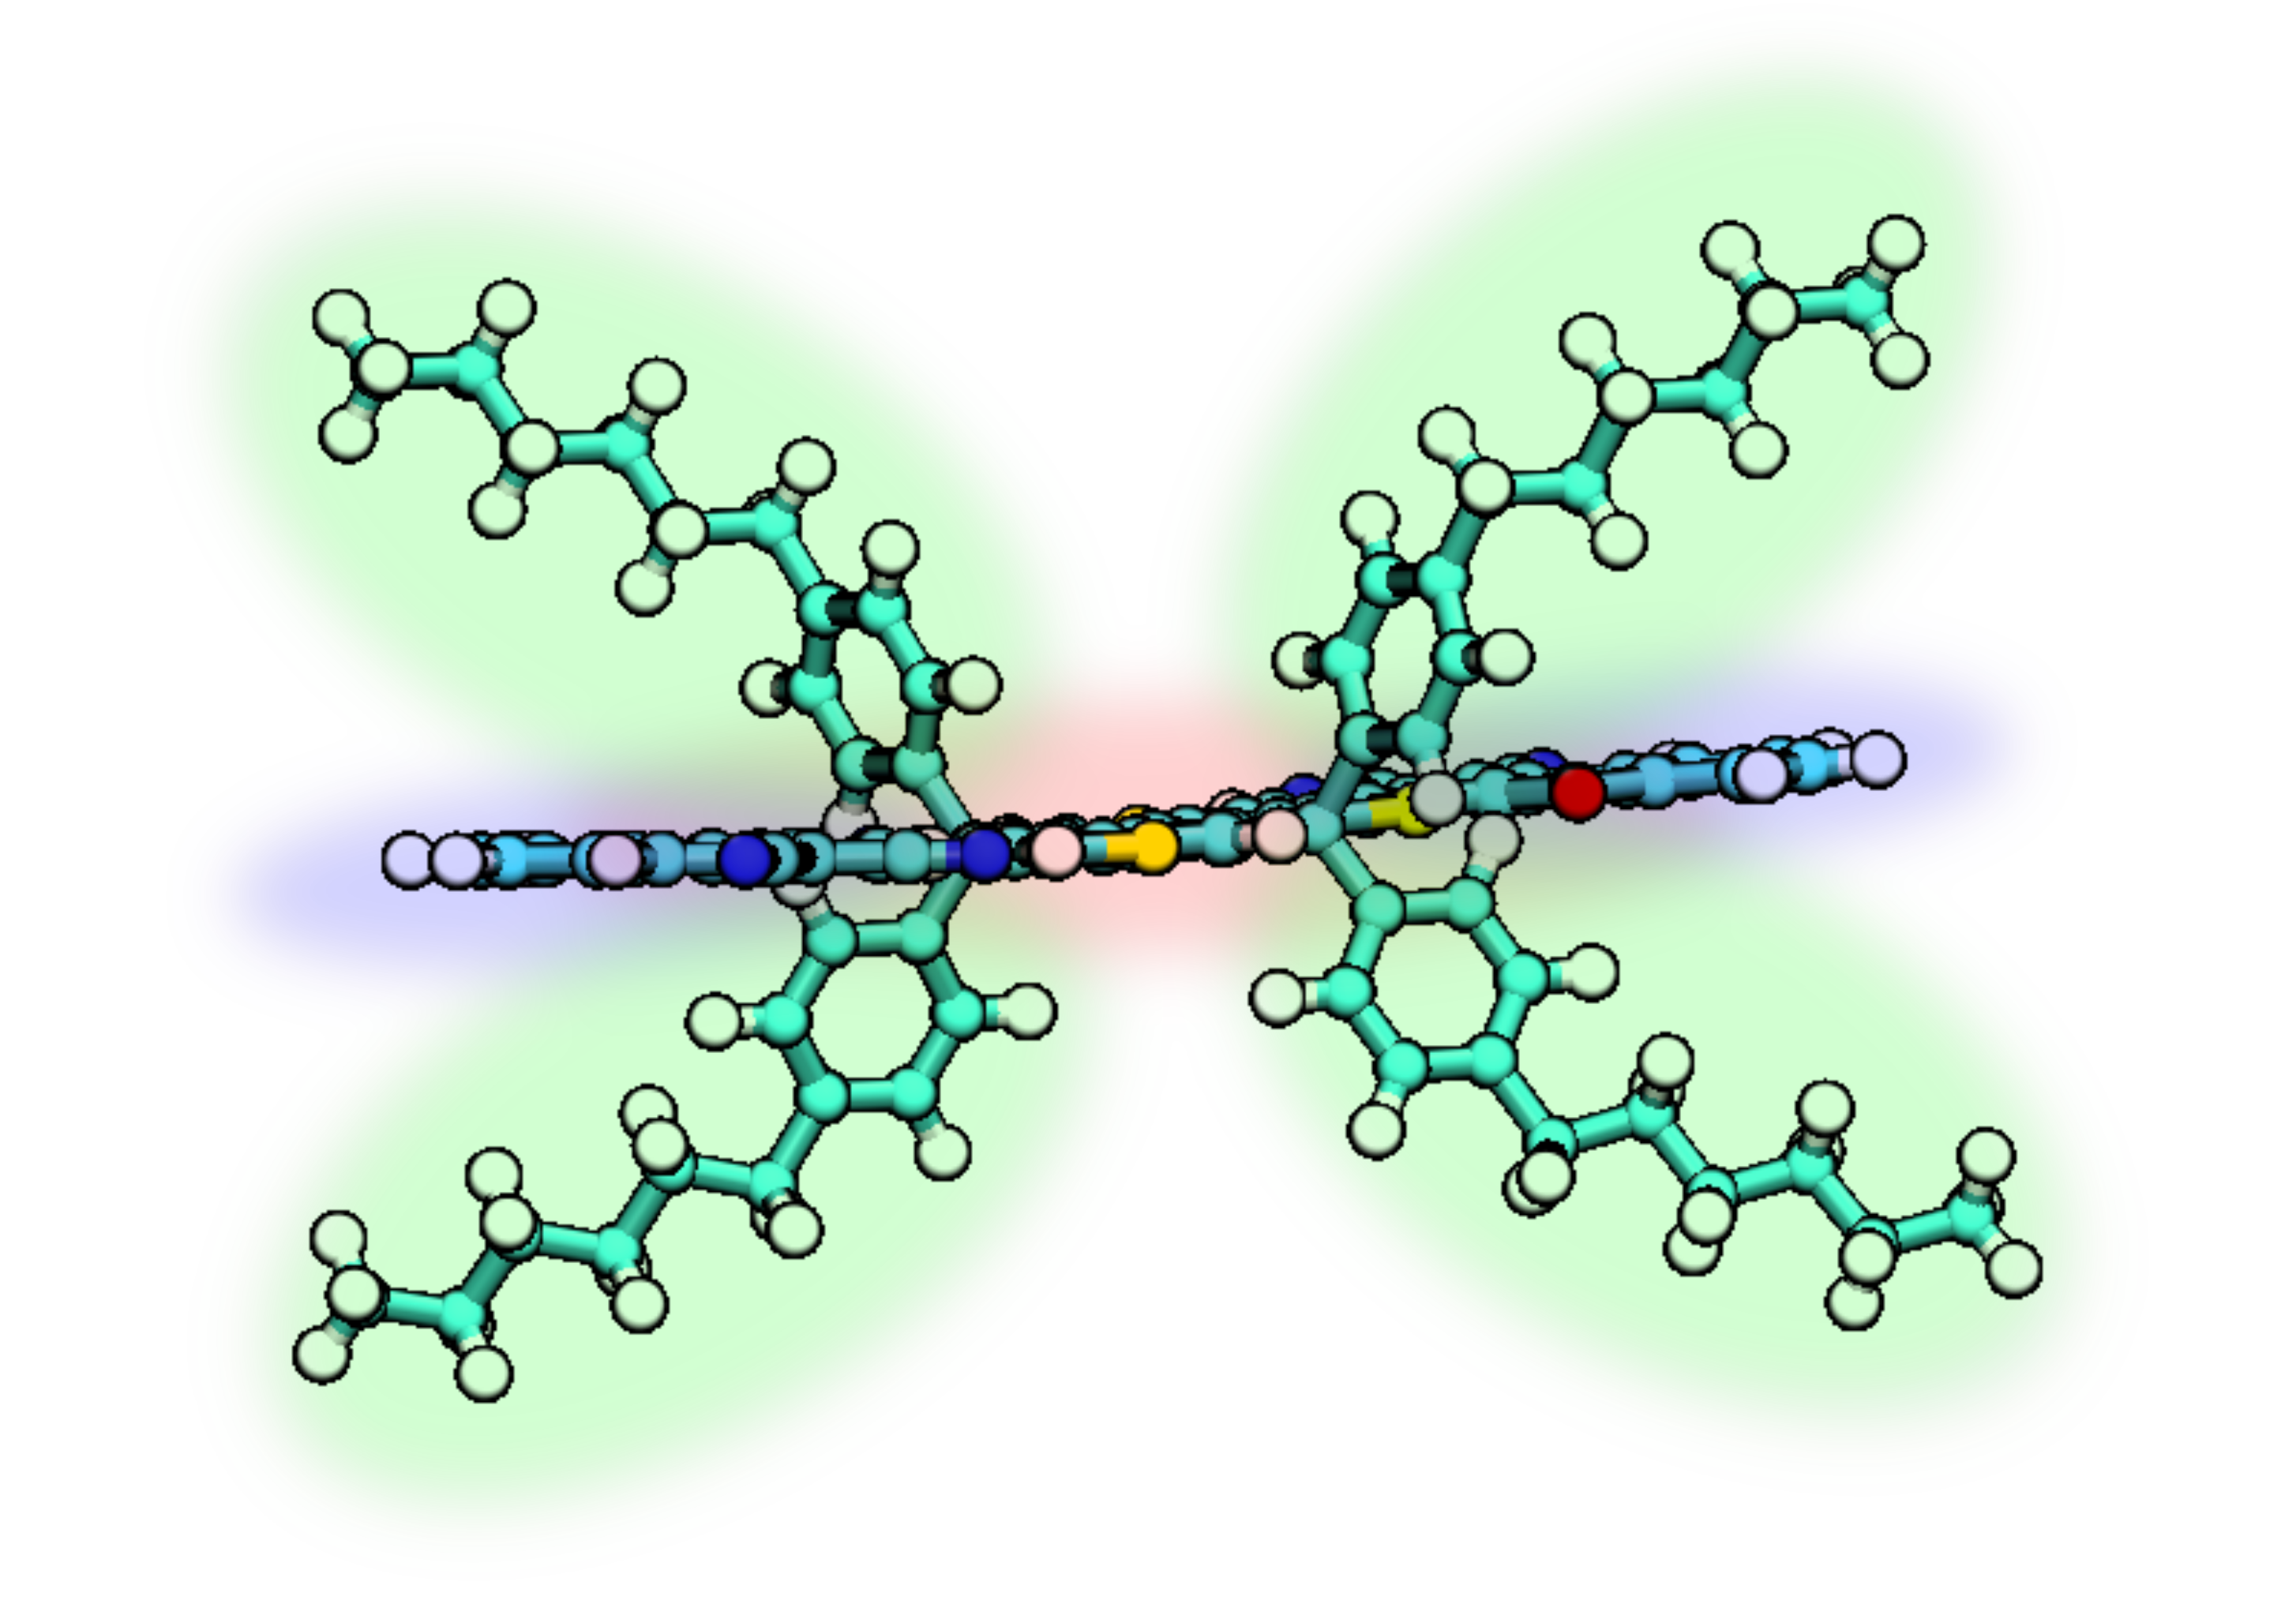
\includegraphics[width=\textwidth]{figures/itic-sidechain-figure.png}
\end{subfigure}
    \caption[]{(A) \glsxtrshort{p3ht} oligomer composed of 15 identical monomers imbued in blue.
    (B) \glsxtrshort{itic} molecule viewed from above the plane of the backbone. 
    (C) \glsxtrshort{itic} viewed in the plane of the backone to show the side chains. \glsxtrshort{itic}
    molecule is imbued with blue, red, and green to call attention to the end groups, fused-ring core, and
    side chains respectively.}
\label{molecules}
\end{figure}

Two \glsxtrshort{opv} materials are studied throughout this thesis.
These are \glsxtrshort{p3ht}, a
donor molecule, and \glsxtrshort{itic}, an acceptor molecule. With respect to organic electronic devices, `acceptors' are the
organic analogue of n-type inorganic semiconductors and `donors' the analogue
of the p-type. We make this note because in the methods we describe a model of
a charge hopping from one molecule to another. And as we describe, our
investigation involves hops within a pure donor domain or within a pure
acceptor domain (not to and from donor and acceptor as would be the case at the interface). 
Any molecule can accept or donate a charge carrier.
They merely receive a donor/acceptor designation as a result of how they
are primarily utilized in electronic devices. 

%need to say more things and cleaner things but im not sure what right now
\glsxtrshort{p3ht} is a polymeric material that is highly polymorphic in that it can self-assemble into a wide spectrum of
crystallinities depending on how it is processed.
Polythiophenes as a whole have been well investigated 
since 1883 when they were first characterized~\cite{Poelking2014}.
Seen in \autoref{ITIC/P3HT}, the molecular structure of \glsxtrshort{p3ht}
is such that these molecules can pi-stack into lamellar structures that facilitate fast charge transport along
the backbones. \glsxtrshort{p3ht} was first synthesized by Rick Mcullough in 1992. The first devices to utilize \glsxtrshort{p3ht} showed
a low mobility do to is regio-randomness inhibiting the lamellar packing exhibited by the now widely used
regio-regular (head-to-tail) \glsxtrshort{p3ht} shown in \autoref{molecules}~\cite{Zaumseil2014}. 

\glsxtrshort{itic} is not polymeric. Rather, it a material consisting of small molecules with no long range bonding.
\glsxtrshort{itic} is a \glsxtrshort{frea} that was first synthesized in 2015~\cite{Bai201U}. The structure of \glsxtrshort{itic} is shown in
\autoref{molecules} wherein we have highlighted the moeities.  

In \autoref{methods}, we
provide an exposition of the theories and software packages used to model and simulate self-assembly and charge mobility in
\glsxtrshort{opv}s.
The methods used in this thesis are centrally motivated by, and justified for, 
the application of our workflow to materials
used in \glsxtrshort{osc} design. However, the methods are
not exclusively applicable to these materials and could be applied similarly to supplement the engineering of any organic
electronic devices, like those mentioned above. 
In \autoref{results}, we use \texttt{MorphCT} to validate our current workflow against a predecessor of the 
workflow on three benchmark MD simulated morpholgies of \glsxtrshort{p3ht}. 
Following that, again using \glsxtrshort{p3ht}, we test the sensitivity of our charge mobility prediction, 
implemented with \texttt{MorphCT}, to various inputs. We conclude \autoref{results} by applying our pipeline,
start to finish, to \glsxtrshort{itic}. 
In \autoref{conclusion}, we outline the ramification of \autoref{results} and detail the areas of future development of the workflow. 

%%THESE SENTECES HAS NO HOME Researchers have to balance the optimiztion of electron structures of candidate donor/acceptor materials against the miscibility of two candidate molecules as well as the resultant morphology across the thermodynamic landscape of variuos solution processes which ultimately govern the Jsc and FF of at the device level \cite{Zhu2020a}. This type of molecular tinkering is a critical first step that can lay the groundwork for further wetlb experiments and can ultimately inform device design. Unfortunately, the molecular modularity of FREAs is not mirrored in the software used to study them. \textit{Ab initio} DFT methods are prohibitivly slow on the nanometer scale. Furthermore, investigations like these rarely publish the code necessary to reproduce or extend thework, and often utilize proprietary software. On the contrary, the software used in this work is maintained in public. In the
%
%% Local Variables: 
%%% mode: latex
%%% TeX-master: "BSUmain"
%%:set textwidth=80
% End: 
